\documentclass{standalone}

%Load necesary libraries
\usepackage{tikz}
\usetikzlibrary{fit, calc, decorations.markings}
\usepackage{geometry}
\geometry{paperwidth=17cm,paperheight=20.5cm}
\usepackage{amsthm,mathtools}
\usepackage{bm}% bold math

\usepackage{xcolor}
\definecolor{oneC}{RGB}{255,0,244}
\definecolor{twoC}{RGB}{0,238,255}
\begin{document}
%		\begin{frame}[shrink=0]
				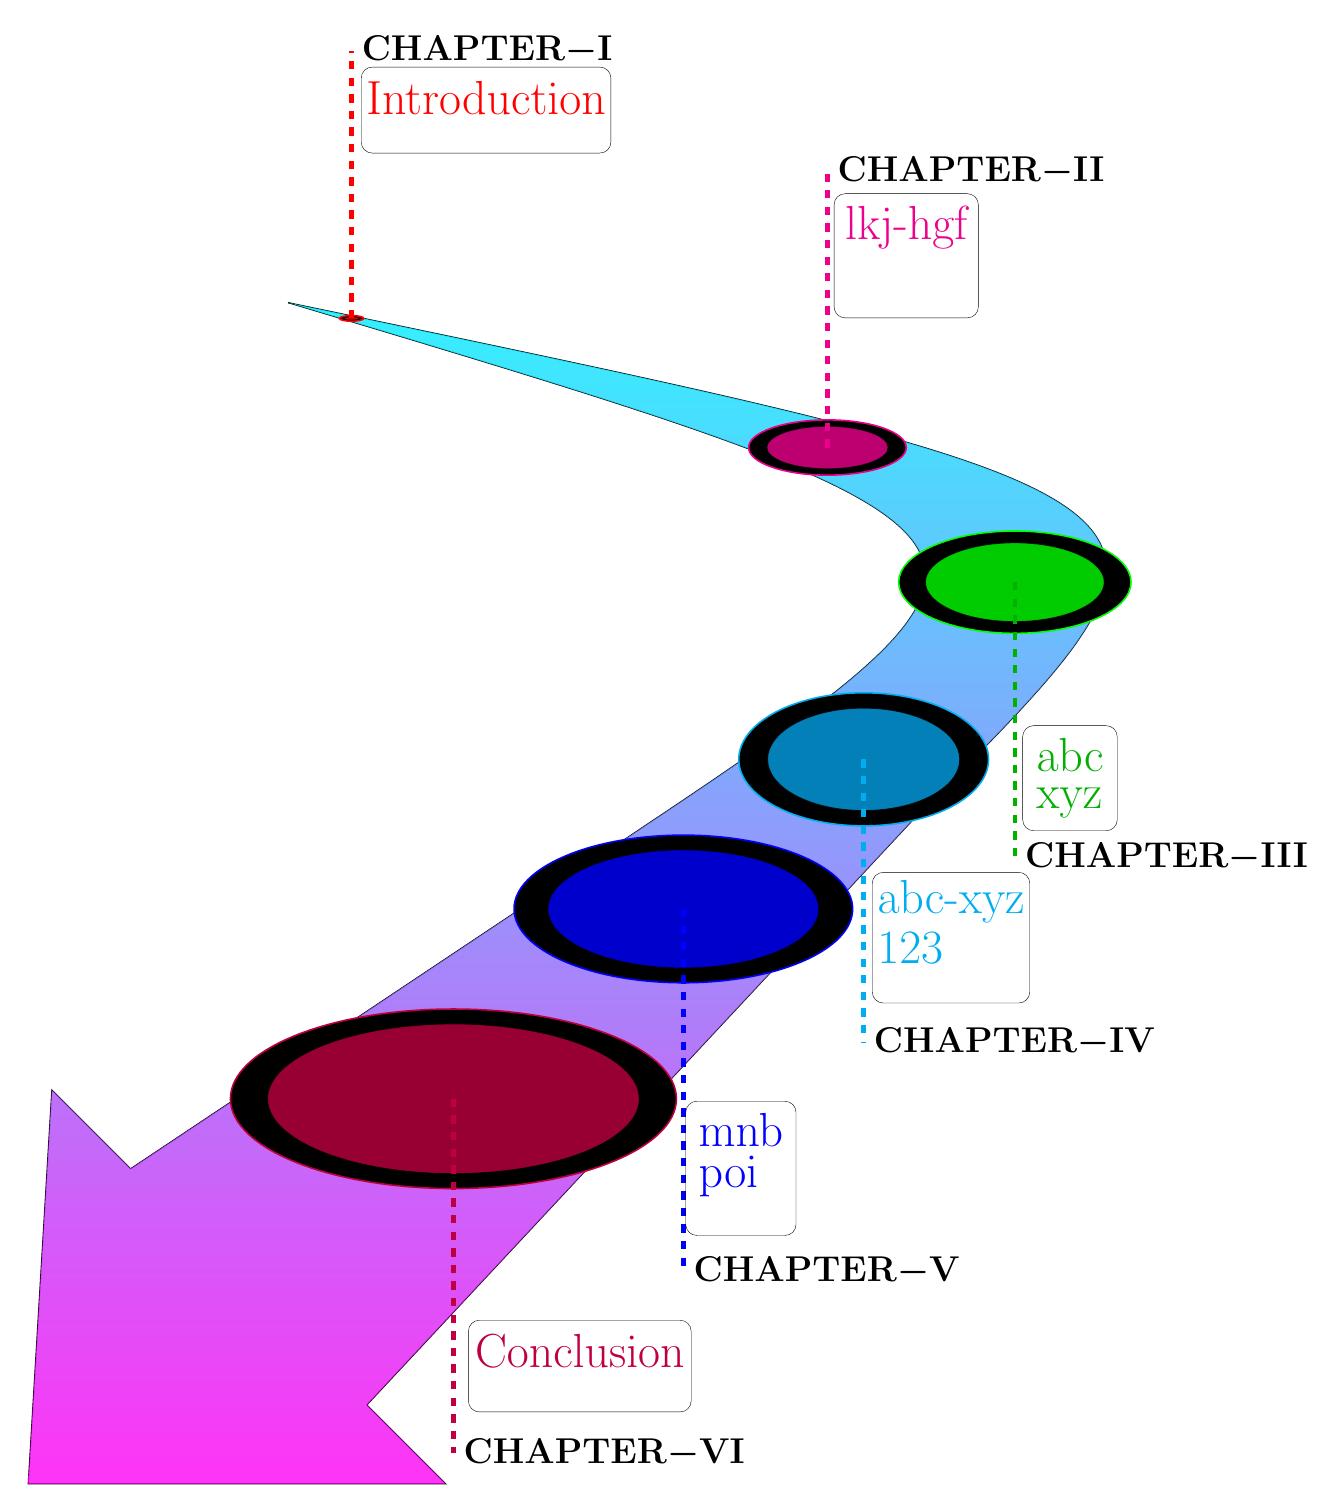
\begin{tikzpicture}%[remember picture, overlay, shift={(8,-3)}]
					
					%Define control points for the first S-shaped curve
					\coordinate (start) at (-4, 0);
					\coordinate (control1) at (6, -3);
					\coordinate (middle) at (0, -7);
					\coordinate (end1) at (-6, -11);
					
					% Draw the first S-shaped curve
					\draw(start) .. controls (control1) .. (middle) .. controls (middle) and (end1) .. (end1);
					
					% Optional: Add labels to the control points for the first curve
					%		\filldraw [olive] (start) circle (3pt) node[left] {\LARGE Objectives};
					%\filldraw [red] (control1) circle (2pt) node[left] {Control 1};
					%\filldraw [red] (middle) circle (2pt) node[above] {Middle};
					%\filldraw [red] (end1) circle (2pt) node[below] {End 1};
					
					% Define control points for the second S-shaped curve
					\coordinate (control3) at (8, -2.5);
					\coordinate (middle2) at (4, -6.5);
					\coordinate (end2) at (-3, -14);
					
					% Draw the second S-shaped curve with an arrow at the end
					\draw (start) .. controls (control3) .. (middle2) .. controls (middle2) and (end2) .. (end2);
					
					% Optional: Add labels to the control points for the second curve
					%\filldraw [blue] (control3) circle (2pt) node[right] {Control 3};
					%\filldraw [blue] (middle2) circle (2pt) node[below] {Middle 2};
					%\filldraw [blue] (end2) circle (2pt) node[above] {End 2};
					
					%General coordinates
					\coordinate (arrow1) at ($(end1) + (-1, +1)$);
					\coordinate (arrow2) at ($(end2) + (+1, -1)$);
					\coordinate (arrow3) at ($(arrow2) + (-5.3, 0)$);
					
					% Optional: Add labels to the control points for the arrow head
					%\filldraw [green] (arrow1) circle (2pt) node[below] {Arrow 1};
					%\filldraw [green] (arrow2) circle (2pt) node[above] {Arrow 2};
					%\filldraw [green] (arrow3) circle (2pt) node[above] {Arrow 3};
					
					%Draw the arrow head
					\draw (end1) -- (arrow1) -- (arrow3) -- (arrow2) -- (end2);
					
					%Shade the region between the two curves
					\begin{scope}
						\shade[bottom color=oneC, top color=twoC, opacity=0.8] 
						(arrow3) -- (arrow2) -- (end2) -- (middle2) .. controls (control3) .. (start) .. controls (control1) .. (middle) .. controls (middle) and (end1) .. (end1) -- (arrow1) -- (arrow3) -- cycle;
					\end{scope}
					
					% Define control points for the curved path
					\coordinate (pathControl) at ($(control1)!0.5!(control3)$);
					\coordinate (pathMiddle) at ($(middle)!0.5!(middle2)$);
					\coordinate (pathEnd) at (arrow3);
					\coordinate (pathEnd2) at ($(end1)!0.5!(end2)$);
					
					% Draw the curved path
					%\filldraw [yellow] (pathControl) circle (2pt) node[below] {Path Control};
					%\filldraw [yellow] (pathMiddle) circle (2pt) node[below] {Path Middle};
					%\filldraw [yellow] (pathEnd) circle (2pt) node[below] {Path End};
					%\filldraw [yellow] (pathEnd2) circle (2pt) node[below] {Path End2};
					%\draw[red] (start) .. controls (pathControl) .. (pathMiddle) .. controls (pathMiddle) and (pathEnd) .. (pathEnd2);
					%\draw[blue] (pathEnd2) -- (pathEnd);
					
					% Draw ovals around the existing ovals with the same ratios
					\draw[color=red, fill=black,fill opacity=1,line width=0.02cm] ($(start) + (0.806, -0.2)$) ellipse [x radius=0.098cm*1.575, y radius=0.0225cm*1.575];
					%		\draw[color=orange, fill=black,fill opacity=1, line width=0.02cm] ($(start) + (4.2, -1.074)$) ellipse [x radius=0.436cm*1.5, y radius=0.155cm*1.5];
					\draw[color = magenta, fill=black,fill opacity=1, line width = 0.02cm] ($(start) + (6.85, -1.84)$) ellipse [x radius=0.77cm*1.3, y radius=0.27cm*1.3];
					\draw[color = green, fill=black,fill opacity=1, line width = 0.02cm] ($(start) +(9.23, -3.55)$) ellipse [x radius=1.135cm*1.3, y radius=0.5cm*1.3];
					\draw[color = cyan, fill=black,fill opacity=1, line width = 0.02cm] ($(start) + (7.31, -5.8)$) ellipse [x radius=1.22cm*1.3, y radius=0.65cm*1.3];
					\draw[color = blue, fill=black,fill opacity=1,line width = 0.02cm] ($(start) + (5.02, -7.7)$) ellipse [x radius=1.72cm*1.25, y radius=0.75cm*1.25];
					\draw[color = purple, fill=black,fill opacity=1,line width = 0.02cm] ($(start) + (2.1, -10.111)$) ellipse [x radius=2.36cm*1.2, y radius=0.95cm*1.2];
					
					% Draw ovals at the starting point
					\draw[color = black, fill = red, opacity = 0.8, line width=0.01cm] ($(start) + (0.806, -0.2)$) ellipse [x radius=0.098cm, y radius=0.0225cm];
					%		\draw[color = black, fill = orange, opacity = 0.8, line width=0.01cm] ($(start) + (4.2, -1.074)$) ellipse [x radius=0.436cm, y radius=0.155cm];
					\draw[color = black, fill = magenta, opacity = 0.8, line width=0.01cm] ($(start) + (6.85, -1.84)$) ellipse [x radius=0.77cm, y radius=0.27cm];
					\draw[color = black, fill = green, opacity = 0.8, line width=0.01cm] ($(start) + (9.23, -3.55)$) ellipse [x radius=1.135cm, y radius=0.5cm];
					\draw[color = black, fill = cyan!90!blue, opacity = 0.8, line width=0.01cm] ($(start) + (7.31, -5.8)$) ellipse [x radius=1.22cm, y radius=0.65cm];
					\draw[color = black, fill = blue, opacity = 0.8, line width=0.01cm] ($(start) + (5.02, -7.7)$) ellipse [x radius=1.72cm, y radius=0.75cm];
					\draw[color = black, fill = purple, opacity = 0.8, line width=0.01cm] ($(start) + (2.1, -10.111)$) ellipse [x radius=2.36cm, y radius=0.95cm];
					
					
					
					% Draw perpendicular lines going up 3cm
					\draw[color = red, ultra thick, dashed, opacity = 1] ($(start) + (0.806, -0.2)$) -- ++(90:3.4cm) node[right, scale = 0.9, color = black] {\Large \textbf{CHAPTER}\bm{$-\mathrm{I}$}};
					%		\draw[color = orange, ultra thick, dashed, opacity = 1] ($(start) + (4.2, -1.074)$) -- ++(90:3.5cm) node[right, scale = 0.9, color = black] {\Large \textbf{CHAPTER}\bm{$-\mathrm{II}$}};
					\draw[color = magenta, ultra thick, dashed, opacity = 1] ($(start) + (6.85, -1.84)$) -- ++(90:3.5cm) node[right, scale = 0.9, color = black] {\Large \textbf{CHAPTER}\bm{$-\mathrm{II}$}};
					\draw[color = green!70!black, ultra thick, dashed, opacity = 1] ($(start) + (9.23, -3.55)$) -- ++(-90:3.5cm)  node[right, scale = 0.9, color = black] {\Large \textbf{CHAPTER}\bm{$-\mathrm{III}$}};
					\draw[color = cyan, ultra thick, dashed, opacity = 1] ($(start) + (7.31, -5.8)$) -- ++(-90:3.6cm) node[right, scale = 0.9, color = black] {\Large \textbf{CHAPTER}\bm{$-\mathrm{IV}$}};
					\draw[color = blue, dashed, opacity = 1, ultra thick] ($(start) + (5.02, -7.7)$) -- ++(-90:4.6cm) node[right, scale = 0.9, color = black] {\Large \textbf{CHAPTER}\bm{$-\mathrm{V}$}};
					\draw[color = purple, ultra thick, dashed, opacity = 1] ($(start) + (2.1, -10.111)$) -- ++(-90:4.5cm) node[right, scale = 0.9, color = black] {\Large \textbf{CHAPTER}\bm{$-\mathrm{VI}$}};
					
					% Add text under the years
					\node[right, color = red, scale = 1] (1) at ($(start) + (0.87, -0.2)  + (90:2.8cm)$) {\LARGE Introduction};
					\node[right, color = black, scale = 1] (2) at ($(start) + (0.87, -0.32)  + (90:2.4cm)$) {\LARGE};
					\node[right, color = orange, scale = 1] (3) at ($(start) + (4.27, -1.074)  + (90:2.8cm)$) {\LARGE};
					\node[right, color = orange, scale = 1] (4) at ($(start) + (4.27, -1.074) + (90:2.2cm)$) {\LARGE};
					\node[right, color = magenta, scale = 1] (5) at ($(start) + (6.95, -1.84) + (90:2.8cm)$) {\LARGE lkj-hgf};
					\node[right, color = magenta, scale = 1] (6) at ($(start) + (6.95, -1.84)+ (90:2.2cm)$) {\LARGE};
					\node[right, color = magenta, scale = 1] (7) at ($(start) + (6.95, -1.84) + (90:1.8cm)$) {\LARGE};
					\node[right, color = green!69!black, scale = 1] (8) at ($(start) + (9.38, -3.55) + (-90:2.2cm)$) {\LARGE abc};
					\node[right, color = green!69!black, scale = 1] (9) at ($(start) + (9.38, -3.55) + (-90:2.8cm)$) {\LARGE xyz};
					\node[right, color = cyan, scale = 1] (10) at ($(start) + (7.36, -5.8) + (-90:1.8cm)$) {\LARGE abc-xyz};
					\node[right, color = cyan, scale = 1] (11) at ($(start) + (7.36, -5.8) + (-90:2.4cm)$) {\LARGE 123};
					\node[right, color = cyan, scale = 1] (12) at ($(start) + (7.36, -5.8) + (-90:3cm)$) {\LARGE };
					\node[right, color = blue, scale = 1] (13) at ($(start) + (5.09, -7.7) + (-90:2.8cm)$) {\LARGE mnb};
					\node[right, color = blue, scale = 1] (14) at ($(start) + (5.09, -7.7) + (-90:3.4cm)$) {\LARGE  poi};
					\node[right, color = blue, scale = 1] (15) at ($(start) + (5.09, -7.7) + (-90:4cm)$) {\LARGE };
					\node[right, color = purple, scale = 1] (16) at ($(start) + (2.25, -10.111) + (-90:3.2cm)$) {\LARGE Conclusion};
					\node[right, color = purple, scale = 1] (17) at ($(start) + (2.25, -10.111) + (-90:3.8cm)$) {};
					
					% Draw a box around the text nodes with the same opacity
					\node[draw, line width = 0.005cm, rounded corners, scale = 0.9, fit={(1) (2)}] {};
					%		\node[draw, line width = 0.005cm, rounded corners, scale = 0.85, fit={(3) (4)}] {};
					\node[draw, line width = 0.005cm, rounded corners, scale = 0.9, fit={(5) (6) (7)}] {};
					\node[draw, line width = 0.005cm, rounded corners, scale = 0.9, fit={(8) (9)}] {};
					\node[draw, line width = 0.005cm, rounded corners, scale = 0.85, fit={(10) (11) (12)}] {};
					\node[draw, line width = 0.005cm, rounded corners, scale = 0.9, fit={(13) (14) (15)}] {};
					\node[draw, line width = 0.005cm, rounded corners, scale = 0.9, fit={(16) (17)}] {};
					
				\end{tikzpicture}

%		\end{frame}	
	\end{document}